\begin{surferIntroPage}{Tutorial}{tutorial_koord1}{Premiers pas avec SURFER}
Ce programme s'appelle SURFER. Quand vous lisez ce mot, vous pensez sûrement à la plage, au soleil et aux vagues. Ici, le nom vient du mot {\it surface}.
\\
Avec SURFER, on peut visualiser des surfaces, et plus précisément des sufaces algébriques. Choisissez une des surfaces à droite pour explorer les différents chapitres de ce tutoriel.\\
SURFER fait partie de l'exposition itinérante IMAGINARY, née à l'occasion de l'Année Allemande des Mathématiques, en 2008. Cette exposition est un projet mené par le Mathematisches Forschungsinstitut Oberwolfach, de renommée internationale, situé dans la Forêt Noire allemande. Chaque semaine ont lieu à l'institut des séminaires sur des sujets récents de la recherche mathématique. Ces séminaires sont importants pour favoriser les échanges entre les scientifiques du monde entier. \\
\vspace{0.2cm} \hspace{3.5cm}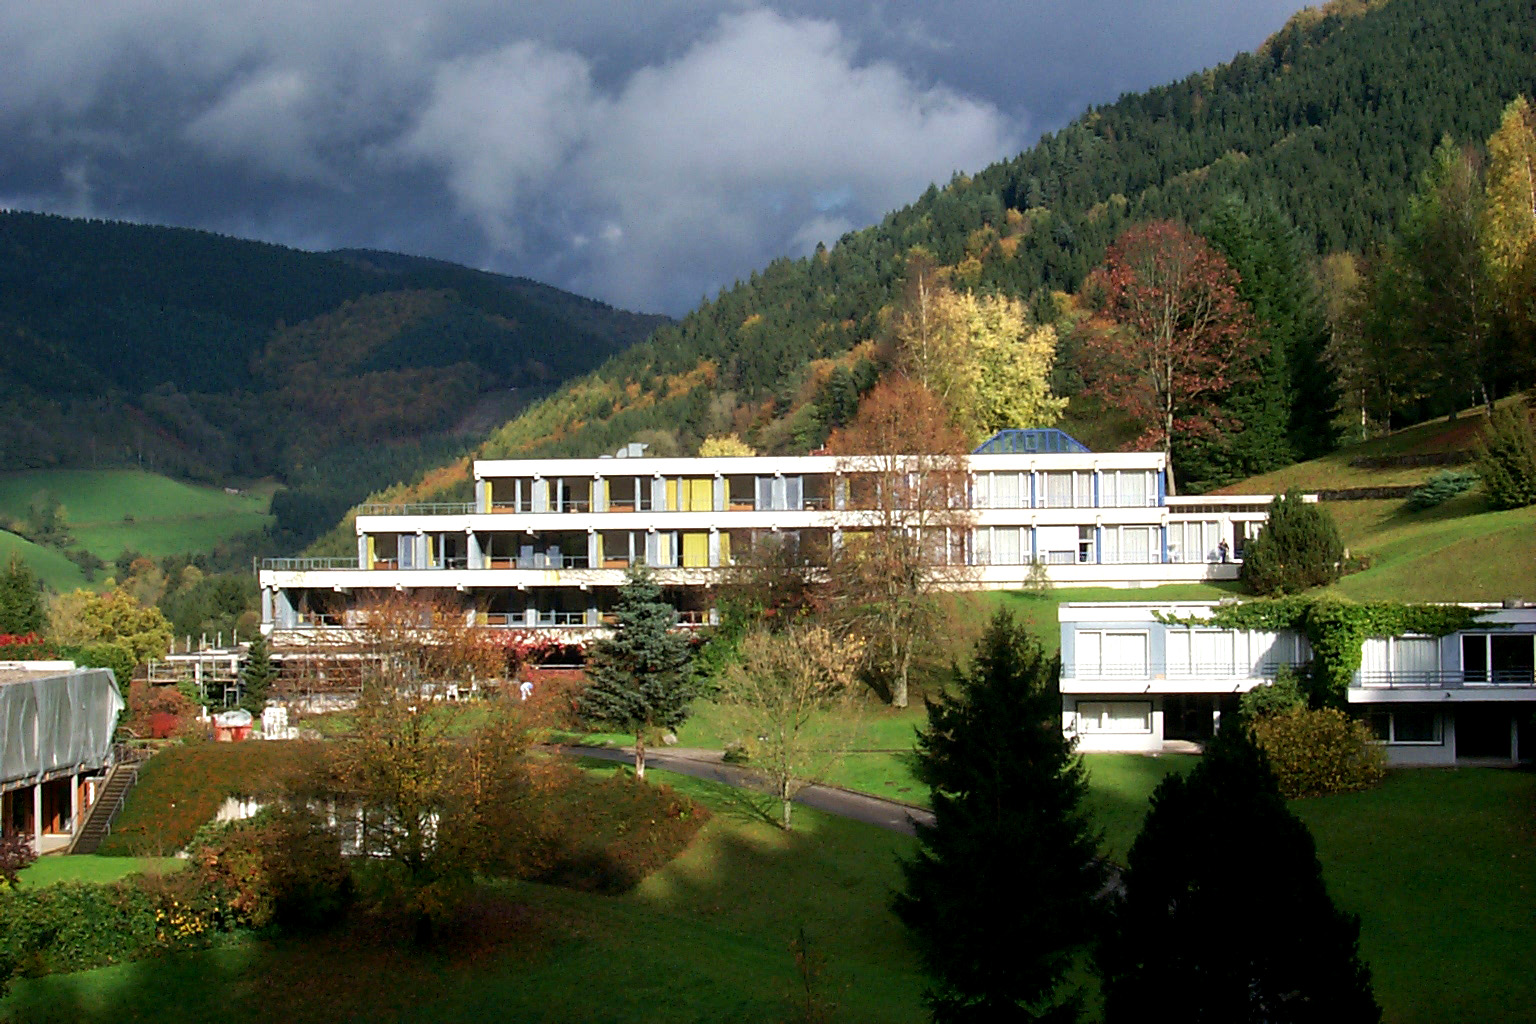
\includegraphics[width=3cm]{./../../common/images/photo_mfo.jpg}\\
Vous pouvez télécharger gratuitement le programme SURFER sur notre page d'accueil :\\
\begin{centering}
www.imaginary.org\\
\end{centering}
 \vspace{0.2cm}
A droite, vous pouvez choisir un des tutoriels mathématiques, en commençant par la surface Zitrus. A votre gauche, vous pouvez naviguer vers d'autres galeries, par exemple celle des surfaces créatives.
\end{surferIntroPage}
